\documentclass{article}
\usepackage{import}
\import{../../../lib/latex/}{wgmlgz}


\begin{document}

\itmo[
  variant=15326,
  labn=3,
  discipline=Основы профессиональной деятельности,
  group=P3115,
  student=Владимир Мацюк,
  teacher=Абузов Ярослав
  Александрович,
  logo=../../../lib/img/itmo.png
]

\section{Текст задания}
По выданному преподавателем варианту восстановить текст заданного варианта программы, определить предназначение и составить описание программы, определить область представления и область допустимых значений исходных данных и результата, выполнить трассировку программы.
\begin{center}
  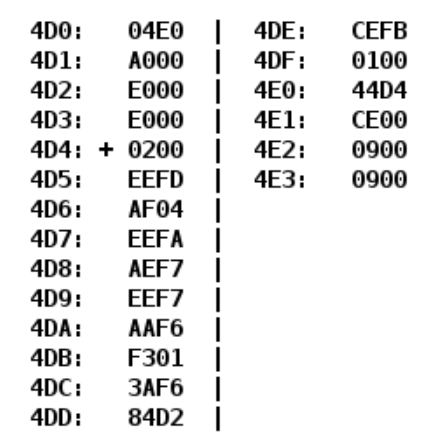
\includegraphics[scale=0.8]{task.png}
\end{center}
\begin{tabular}{|c|r|l|l|} \hline
  Адрес & Код команды & Мнемоника  & Комментарии \nl
  4D0   & 04E0        & a          & \nl
  4D1   & A000        & b          & \nl
  4D2   & E000        & n          & \nl
  4D3   & E000        & r          & \nl
  4D4   & +0200       & CLA        & Очистка аккумулятора\nl
  4D5   & EEFD        & ST IP-3    & (r)Сохранение (Прямая относительная адресация)\nl
  4D6   & AF04        & LD 0x04    & Загрузка (Прямая загрузка операнда)\nl
  4D7   & EEFA        & ST IP-6    & (n) Сохранение (Прямая относительная адресация)\nl
  4D8   & AEF7        & LD IP-9    & (a) Загрузка (Прямая относительная адресация)\nl
  4D9   & EEF7        & ST IP-9    & (b) Сохранение (Прямая относительная адресация)\nl

  4DA   & AAF6        & LD (IP-A)+ & (b) loop: Загрузка (Косвенная относительная автоинкрементная адресация)\nl
  4DB   & F301        & BPL IP+1   & Переход, если плюс\nl
  4DC   & 3AF6        & OR (IP-A)+ & (r) Логическое или (Косвенная относительная автоинкрементная адресация)\nl
  4DD   & 84D2        & LOOP 0x4D2 & (n) Декремент и пропуск (Прямая абсолютная адресация)\nl
  4DE   & CEFB        & JUMP IP-5    & Безусловный переход (loop) (прямая относительная адресация)\nl
  4DF   & 0100        & HLT        & Остановка\nl
  4E0   & 44D4        & arr[0]     & \nl
  4E1   & CE00        & arr[1]     & \nl
  4E2   & 0900        & arr[2]     & \nl
  4E3   & 0900        & arr[3]     & \nl
\end{tabular}

\section{Описание программы}

Программа находит количесво отрицательных чисел и сохраняет результат в ячейке 4D3.
Псевдокод:

\begin{lstlisting}
a = 0x4e0
b = a
n = 4
r = 0

do {
  ac = *(b++)
  if ac <= 0 {
    ac |= *(r++)
  }
} while (--n > 0)

  
\end{lstlisting}


\section{Область представления}
\begin{itemize}
  \item a, b – 11-ти разрядные, адрес БЭВМ.
  \item r, n – 16-ти разрядные целые, беззнаковое.
  \item arr[i] – 16-ти разрядные знаковые целые числа.
\end{itemize}
\section{Область допустимых значений}

\begin{itemize}
  \item $ n \in [1;  2^{11} - 4e0_{16}] = [1; 800]\ |\ [1, 4CF_{16}]$ 1 т.к. цикл выполнится как минимум 1 раз
  \item $ r \in [0;  n] $
  \item $ a, b \in [4e0_{16};  2^{11}]\ |\ [0;  4CF_{16}] $
  \item $arr[i] \in [-2^{15}; 2^{15}-1]$
\end{itemize}

\section{Расположение данных в памяти}

\begin{itemize}
  \item 4E0, 4E1, 4E2, 4E3 – исходные данные;
  \item  4D0, 4D1, 4D2, 4D3 – промежуточные значения;
  \item  4D4 – 4DF – команды
\end{itemize}

\section{Адреса первой и последней выполняемой команды}

\begin{itemize}
  \item Адрес первой команды: 4D4
  \item Адрес последней команды: 4Df
\end{itemize}
\section{Таблица трассировки}

\begin{tabular}{|c|c|c|c|c|c|c|c|c|c|c|c|c|c|c|} \hline
  Адр & Код  & IP  & CR   & AR  & DR   & SP  & BR   & AC   & PS  & NZVC & Адр & Код \nl
  4D4 & 0200 & 4D4 & 0000 & 000 & 0000 & 000 & 0000 & 0000 & 004 & 0100 &     & \nl
  4D4 & 0200 & 4D5 & 0200 & 4D4 & 0200 & 000 & 04D4 & 0000 & 004 & 0100 &     & \nl
  4D5 & EEFD & 4D6 & EEFD & 4D3 & 0000 & 000 & FFFD & 0000 & 004 & 0100 & 4D3 & 0000 \nl
  4D6 & AF04 & 4D7 & AF04 & 4D6 & 0004 & 000 & 0004 & 0004 & 000 & 0000 &     & \nl
  4D7 & EEFA & 4D8 & EEFA & 4D2 & 0004 & 000 & FFFA & 0004 & 000 & 0000 & 4D2 & 0004 \nl
  4D8 & AEF7 & 4D9 & AEF7 & 4D0 & 04E0 & 000 & FFF7 & 04E0 & 000 & 0000 &     & \nl
  4D9 & EEF7 & 4DA & EEF7 & 4D1 & 04E0 & 000 & FFF7 & 04E0 & 000 & 0000 & 4D1 & 04E0 \nl

  4DA & AAF6 & 4DB & AAF6 & 4E0 & 44D4 & 000 & FFF6 & 44D4 & 000 & 0000 & 4D1 & 04E1 \nl
  4DB & F301 & 4DD & F301 & 4DB & F301 & 000 & 0001 & 44D4 & 000 & 0000 &     & \nl
  4DD & 84D2 & 4DE & 84D2 & 4D2 & 0003 & 000 & 0002 & 44D4 & 000 & 0000 & 4D2 & 0003 \nl
  4DE & CEFB & 4DA & CEFB & 4DE & 04DA & 000 & FFFB & 44D4 & 000 & 0000 &     & \nl

  4DA & AAF6 & 4DB & AAF6 & 4E1 & CE00 & 000 & FFF6 & CE00 & 008 & 1000 & 4D1 & 04E2 \nl
  4DB & F301 & 4DC & F301 & 4DB & F301 & 000 & 04DB & CE00 & 008 & 1000 &     & \nl
  4DC & 3AF6 & 4DD & 3AF6 & 000 & 0000 & 000 & 31FF & CE00 & 008 & 1000 & 4D3 & 0001 \nl
  4DD & 84D2 & 4DE & 84D2 & 4D2 & 0002 & 000 & 0001 & CE00 & 008 & 1000 & 4D2 & 0002 \nl
  4DE & CEFB & 4DA & CEFB & 4DE & 04DA & 000 & FFFB & CE00 & 008 & 1000 &     & \nl

  4DA & AAF6 & 4DB & AAF6 & 4E2 & 0900 & 000 & FFF6 & 0900 & 000 & 0000 & 4D1 & 04E3 \nl
  4DB & F301 & 4DD & F301 & 4DB & F301 & 000 & 0001 & 0900 & 000 & 0000 &     & \nl
  4DD & 84D2 & 4DE & 84D2 & 4D2 & 0001 & 000 & 0000 & 0900 & 000 & 0000 & 4D2 & 0001 \nl
  4DE & CEFB & 4DA & CEFB & 4DE & 04DA & 000 & FFFB & 0900 & 000 & 0000 &     & \nl

  4DA & AAF6 & 4DB & AAF6 & 4E3 & 0900 & 000 & FFF6 & 0900 & 000 & 0000 & 4D1 & 04E4 \nl
  4DB & F301 & 4DD & F301 & 4DB & F301 & 000 & 0001 & 0900 & 000 & 0000 &     & \nl
  4DD & 84D2 & 4DF & 84D2 & 4D2 & 0000 & 000 & FFFF & 0900 & 000 & 0000 & 4D2 & 0000 \nl
  4DF & 0100 & 4E0 & 0100 & 4DF & 0100 & 000 & 04DF & 0900 & 000 & 0000 &     & \nl
\end{tabular}

\section{Вывод}

Во время выполнения лабораторной работы я научился работать в БЭВМ с массивами,
ветвлением и циклами. Я изучил прямую и косвенную адресацию и цикл выполнения
таких команд, как LOOP и JUMP.

\end{document}
